\section{Modelling the problem} \label{sec:model}

When constructing autonomous robots like the \projname{}, a few techniques exist to model the robot's known world. It is also important to know what exactly makes an autonomous robot, autonomous. In order for a robot to be autonomous it should be able to make decisions based on the current state the robot is in, previous experiences, and according to the goals that need to be accomplished~\citep{artificialintelligencebook}. 

\begin{figure}[H]
     \center{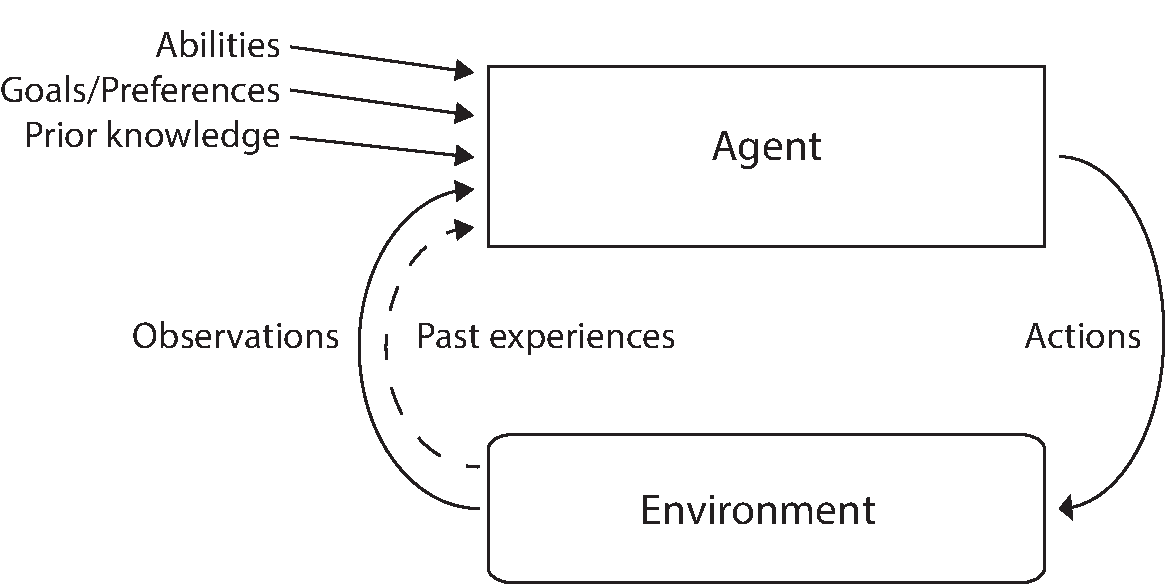
\includegraphics[scale=0.5]
     {graphics/AgentModel.pdf}}
     \caption{\label{fig:model_mi_agent} An agent in an environment.}
\end{figure}

\figref{fig:model_mi_agent} shows an agent, something that acts in an environment, what prior knowledge this agent has and what actions the agent can do to interact with the environment. The \projname{} has the following capabilities:

\begin{description}
\item[Abilities] Abilities are the actions the agent can use to interact with the world. The \projname{} is able to move around the environment by driving forward, backwards and turning. It can sense objects and detect the environment boundaries. It is also able to pickup objects and place these into the attached storage container.  
\item[Goals/Preferences] Goals are the objectives that the agent must complete. The \projname{} should be able to collect all the objects inside the environment within reasonable time. In this project reasonable time is defined to 30 seconds per object. Preferences are rules for which action the robot performs, if two different actions are available and neither necessarily moves it closer to the goal. For instance, which way the robot should turn when it encounters a boundary.
\item[Prior knowledge] The robot will not have any knowledge about the environment beforehand. Other than the programmed logic, it will only know how many objects to collect before halting.
\item[Observations] Knowledge about the current environment. This is obtained by sensors and knowledge of how far the \projname{} has driven. 
\item[Past experiences] Knowledge about how many objects has been collected. 
\end{description}

Despite sounding similar, there is a slight difference between prior knowledge and past experience. The difference is that prior knowledge is information that has been hard coded into the robot, while past experience is something it has learnt by itself. The only past experience \projname{} is collecting is how many objects it has found so far. If it had kept knowledge about previous runs and used it to try and find the new objects faster, it would have been machine learning, which is chosen not to be a part of this project.

In order for the robot to understand the world, it must contain a suitable representation. There are three different ways to represent a world - \emph{State-based}, \emph{Feature-based} and \emph{Relational}~\citep{artificialintelligencebook}. Each of these are shortly discussed and the most suitable is used to model the problem. 

\begin{description}
\item[State-based] In a state-based representation, each state represents a possible model of the world. If the entire environment, i.e. knowledge about the boundary, location of the robot, and object position, should be described using a state-based representation, then a  tremendous amounts of states would be needed to provide the necessary information. The world should also be big enough to precisely place the objects and contain the space in between these. 

A slightly altered version of the state-based representation would be to have a state for each phase of the \projname{}'s behaviour. These states could, for instance, be a \emph{Searching for objects} or \emph{Collecting objects} states. This would greatly decrease the amount of states needed, and still make a state-based representation possible. 

\item[Feature-based] In a feature-based representation, every state can be described in terms of features, where a feature has a value in each state. The entire environment can be represented with a two-dimensional array, in the feature based representation. Each point describes a spot in the environment, where either an object is located, boundary is spotted, or if nothing is in that spot. 

\item[Relational] A relational representation deals with relational descriptions in terms of individuals and relations among them. This can be used to describe states of individuals or their position compared to others. 
\end{description}

Both a state-based and a feature-based representation of the world suits the project. The feature-based representation, where the entire environment would have to be mapped, would require a lot of memory to initialise and update the representation continuously. This would also require that the sensors are accurate enough to find the correct position of the objects. The simple state-based model, by using phases, would be a possible solution for the \projname{} as well. 

